% !TeX TXS-program:bibliography = txs:///biber
\documentclass[14pt, russian]{scrartcl}
\let\counterwithout\relax
\let\counterwithin\relax
%\usepackage{lmodern}
\usepackage{float}
\usepackage{xcolor}
\usepackage{extsizes}
\usepackage{subfig}
\usepackage[export]{adjustbox}
\usepackage{tocvsec2} % возможность менять учитываемую глубину разделов в оглавлении
\usepackage[subfigure]{tocloft}
\usepackage[newfloat]{minted}
\captionsetup[listing]{position=top}

\AtBeginEnvironment{figure}{\vspace{0.5cm}}
\AtBeginEnvironment{table}{\vspace{0.5cm}}
\AtBeginEnvironment{listing}{\vspace{0.5cm}}
\AtBeginEnvironment{algorithm}{\vspace{0.5cm}}
\AtBeginEnvironment{minted}{\vspace{-0.5cm}}

\usepackage{fancyvrb}
\usepackage{ulem,bm,mathrsfs,ifsym} %зачеркивания, особо жирный стиль и RSFS начертание
\usepackage{sectsty} % переопределение стилей подразделов
%%%%%%%%%%%%%%%%%%%%%%%

%%% Поля и разметка страницы %%%
\usepackage{pdflscape}                              % Для включения альбомных страниц
\usepackage{geometry}                               % Для последующего задания полей
\geometry{a4paper,tmargin=2cm,bmargin=2cm,lmargin=3cm,rmargin=1cm} % тоже самое, но лучше

%%% Математические пакеты %%%
\usepackage{amsthm,amsfonts,amsmath,amssymb,amscd}  % Математические дополнения от AMS
\usepackage{mathtools}                              % Добавляет окружение multlined
\usepackage[perpage]{footmisc}
%\usepackage{times}

%%%% Установки для размера шрифта 14 pt %%%%
%% Формирование переменных и констант для сравнения (один раз для всех подключаемых файлов)%%
%% должно располагаться до вызова пакета fontspec или polyglossia, потому что они сбивают его работу
%\newlength{\curtextsize}
%\newlength{\bigtextsize}
%\setlength{\bigtextsize}{13pt}
\KOMAoptions{fontsize=14pt}

\makeatletter
\def\showfontsize{\f@size{} point}
\makeatother

%\makeatletter
%\show\f@size                                       % неплохо для отслеживания, но вызывает стопорение процесса, если документ компилируется без команды  -interaction=nonstopmode
%\setlength{\curtextsize}{\f@size pt}
%\makeatother

%шрифт times
\usepackage{tempora}
%\usepackage{pscyr}
%\setmainfont[Ligatures={TeX,Historic}]{Times New Roman}

   %%% Решение проблемы копирования текста в буфер кракозябрами
%    \input glyphtounicode.tex
%    \input glyphtounicode-cmr.tex %from pdfx package
%    \pdfgentounicode=1
    \usepackage{cmap}                               % Улучшенный поиск русских слов в полученном pdf-файле
    \usepackage[T1]{fontenc}                       % Поддержка русских букв
    \usepackage[utf8]{inputenc}                     % Кодировка utf8
    \usepackage[english, main=russian]{babel}            % Языки: русский, английский
%   \IfFileExists{pscyr.sty}{\usepackage{pscyr}}{}  % Красивые русские шрифты
%\renewcommand{\rmdefault}{ftm}
%%% Оформление абзацев %%%
\usepackage{indentfirst}                            % Красная строка
%\usepackage{eskdpz}

%%% Таблицы %%%
\usepackage{longtable}                              % Длинные таблицы
\usepackage{multirow,makecell,array}                % Улучшенное форматирование таблиц
\usepackage{booktabs}                               % Возможность оформления таблиц в классическом книжном стиле (при правильном использовании не противоречит ГОСТ)

%%% Общее форматирование
\usepackage{soulutf8}                               % Поддержка переносоустойчивых подчёркиваний и зачёркиваний
\usepackage{icomma}                                 % Запятая в десятичных дробях



%%% Изображения %%%
\usepackage{graphicx}                               % Подключаем пакет работы с графикой
\usepackage{wrapfig}

\usepackage{tikz}
\usetikzlibrary{shapes.misc}
\usetikzlibrary{trees}

%%% Списки %%%
\usepackage{enumitem}

%%% Подписи %%%
\usepackage{caption}                                % Для управления подписями (рисунков и таблиц) % Может управлять номерами рисунков и таблиц с caption %Иногда может управлять заголовками в списках рисунков и таблиц
%% Использование:
%\begin{table}[h!]\ContinuedFloat - чтобы не переключать счетчик
%\captionsetup{labelformat=continued}% должен стоять до самого caption
%\caption{}
% либо ручками \caption*{Продолжение таблицы~\ref{...}.} :)

%%% Интервалы %%%
\addto\captionsrussian{%
  \renewcommand{\listingname}{Листинг}%
}
%%% Счётчики %%%
\usepackage[figure,table,section]{totalcount}               % Счётчик рисунков и таблиц
\DeclareTotalCounter{lstlisting}
\usepackage{totcount}                               % Пакет создания счётчиков на основе последнего номера подсчитываемого элемента (может требовать дважды компилировать документ)
\usepackage{totpages}                               % Счётчик страниц, совместимый с hyperref (ссылается на номер последней страницы). Желательно ставить последним пакетом в преамбуле

%%% Продвинутое управление групповыми ссылками (пока только формулами) %%%
%% Кодировки и шрифты %%%

%   \newfontfamily{\cyrillicfont}{Times New Roman}
%   \newfontfamily{\cyrillicfonttt}{CMU Typewriter Text}
	%\setmainfont{Times New Roman}
	%\newfontfamily\cyrillicfont{Times New Roman}
	%\setsansfont{Times New Roman}                    %% задаёт шрифт без засечек
%	\setmonofont{Liberation Mono}               %% задаёт моноширинный шрифт
%    \IfFileExists{pscyr.sty}{\renewcommand{\rmdefault}{ftm}}{}
%%% Интервалы %%%
%linespread-реализация ближе к реализации полуторного интервала в ворде.
%setspace реализация заточена под шрифты 10, 11, 12pt, под остальные кегли хуже, но всё же ближе к типографской классике.
\linespread{1.3}                    % Полуторный интервал (ГОСТ Р 7.0.11-2011, 5.3.6)
%\renewcommand{\@biblabel}[1]{#1}

%%% Гиперссылки %%%
\usepackage{hyperref}

%%% Выравнивание и переносы %%%
\sloppy                             % Избавляемся от переполнений
\clubpenalty=10000                  % Запрещаем разрыв страницы после первой строки абзаца
\widowpenalty=10000                 % Запрещаем разрыв страницы после последней строки абзаца

\makeatletter % малые заглавные, small caps shape
\let\@@scshape=\scshape
\renewcommand{\scshape}{%
  \ifnum\strcmp{\f@series}{bx}=\z@
    \usefont{T1}{cmr}{bx}{sc}%
  \else
    \ifnum\strcmp{\f@shape}{it}=\z@
      \fontshape{scsl}\selectfont
    \else
      \@@scshape
    \fi
  \fi}
\makeatother

%%% Подписи %%%
%\captionsetup{%
%singlelinecheck=off,                % Многострочные подписи, например у таблиц
%skip=2pt,                           % Вертикальная отбивка между подписью и содержимым рисунка или таблицы определяется ключом
%justification=centering,            % Центрирование подписей, заданных командой \caption
%}
%%%        Подключение пакетов                 %%%
\usepackage{ifthen}                 % добавляет ifthenelse
%%% Инициализирование переменных, не трогать!  %%%
\newcounter{intvl}
\newcounter{otstup}
\newcounter{contnumeq}
\newcounter{contnumfig}
\newcounter{contnumtab}
\newcounter{pgnum}
\newcounter{bibliosel}
\newcounter{chapstyle}
\newcounter{headingdelim}
\newcounter{headingalign}
\newcounter{headingsize}
\newcounter{tabcap}
\newcounter{tablaba}
\newcounter{tabtita}
%%%%%%%%%%%%%%%%%%%%%%%%%%%%%%%%%%%%%%%%%%%%%%%%%%

%%% Область упрощённого управления оформлением %%%

%% Интервал между заголовками и между заголовком и текстом
% Заголовки отделяют от текста сверху и снизу тремя интервалами (ГОСТ Р 7.0.11-2011, 5.3.5)
\setcounter{intvl}{3}               % Коэффициент кратности к размеру шрифта

%% Отступы у заголовков в тексте
\setcounter{otstup}{0}              % 0 --- без отступа; 1 --- абзацный отступ

%% Нумерация формул, таблиц и рисунков
\setcounter{contnumeq}{1}           % Нумерация формул: 0 --- пораздельно (во введении подряд, без номера раздела); 1 --- сквозная нумерация по всей диссертации
\setcounter{contnumfig}{1}          % Нумерация рисунков: 0 --- пораздельно (во введении подряд, без номера раздела); 1 --- сквозная нумерация по всей диссертации
\setcounter{contnumtab}{1}          % Нумерация таблиц: 0 --- пораздельно (во введении подряд, без номера раздела); 1 --- сквозная нумерация по всей диссертации

%% Оглавление
\setcounter{pgnum}{0}               % 0 --- номера страниц никак не обозначены; 1 --- Стр. над номерами страниц (дважды компилировать после изменения)

%% Библиография
\setcounter{bibliosel}{1}           % 0 --- встроенная реализация с загрузкой файла через движок bibtex8; 1 --- реализация пакетом biblatex через движок biber

%% Текст и форматирование заголовков
\setcounter{chapstyle}{1}           % 0 --- разделы только под номером; 1 --- разделы с названием "Глава" перед номером
\setcounter{headingdelim}{1}        % 0 --- номер отделен пропуском в 1em или \quad; 1 --- номера разделов и приложений отделены точкой с пробелом, подразделы пропуском без точки; 2 --- номера разделов, подразделов и приложений отделены точкой с пробелом.

%% Выравнивание заголовков в тексте
\setcounter{headingalign}{0}        % 0 --- по центру; 1 --- по левому краю

%% Размеры заголовков в тексте
\setcounter{headingsize}{0}         % 0 --- по ГОСТ, все всегда 14 пт; 1 --- пропорционально изменяющийся размер в зависимости от базового шрифта

%% Подпись таблиц
\setcounter{tabcap}{0}              % 0 --- по ГОСТ, номер таблицы и название разделены тире, выровнены по левому краю, при необходимости на нескольких строках; 1 --- подпись таблицы не по ГОСТ, на двух и более строках, дальнейшие настройки:
%Выравнивание первой строки, с подписью и номером
\setcounter{tablaba}{2}             % 0 --- по левому краю; 1 --- по центру; 2 --- по правому краю
%Выравнивание строк с самим названием таблицы
\setcounter{tabtita}{1}             % 0 --- по левому краю; 1 --- по центру; 2 --- по правому краю

%%% Рисунки %%%
\DeclareCaptionLabelSeparator*{emdash}{~--- }             % (ГОСТ 2.105, 4.3.1)
\captionsetup[figure]{labelsep=emdash,font=onehalfspacing,position=bottom}

%%% Таблицы %%%
\ifthenelse{\equal{\thetabcap}{0}}{%
    \newcommand{\tabcapalign}{\raggedright}  % по левому краю страницы или аналога parbox
}

\ifthenelse{\equal{\thetablaba}{0} \AND \equal{\thetabcap}{1}}{%
    \newcommand{\tabcapalign}{\raggedright}  % по левому краю страницы или аналога parbox
}

\ifthenelse{\equal{\thetablaba}{1} \AND \equal{\thetabcap}{1}}{%
    \newcommand{\tabcapalign}{\centering}    % по центру страницы или аналога parbox
}

\ifthenelse{\equal{\thetablaba}{2} \AND \equal{\thetabcap}{1}}{%
    \newcommand{\tabcapalign}{\raggedleft}   % по правому краю страницы или аналога parbox
}

\ifthenelse{\equal{\thetabtita}{0} \AND \equal{\thetabcap}{1}}{%
    \newcommand{\tabtitalign}{\raggedright}  % по левому краю страницы или аналога parbox
}

\ifthenelse{\equal{\thetabtita}{1} \AND \equal{\thetabcap}{1}}{%
    \newcommand{\tabtitalign}{\centering}    % по центру страницы или аналога parbox
}

\ifthenelse{\equal{\thetabtita}{2} \AND \equal{\thetabcap}{1}}{%
    \newcommand{\tabtitalign}{\raggedleft}   % по правому краю страницы или аналога parbox
}

\DeclareCaptionFormat{tablenocaption}{\tabcapalign #1\strut}        % Наименование таблицы отсутствует
\ifthenelse{\equal{\thetabcap}{0}}{%
    \DeclareCaptionFormat{tablecaption}{\tabcapalign #1#2#3}
    \captionsetup[table]{labelsep=emdash}                       % тире как разделитель идентификатора с номером от наименования
}{%
    \DeclareCaptionFormat{tablecaption}{\tabcapalign #1#2\par%  % Идентификатор таблицы на отдельной строке
        \tabtitalign{#3}}                                       % Наименование таблицы строкой ниже
    \captionsetup[table]{labelsep=space}                        % пробельный разделитель идентификатора с номером от наименования
}
\captionsetup[table]{format=tablecaption,singlelinecheck=off,font=onehalfspacing,position=top,skip=-5pt}  % многострочные наименования и прочее
\DeclareCaptionLabelFormat{continued}{Продолжение таблицы~#2}
\setlength{\belowcaptionskip}{.2cm}
\setlength{\intextsep}{0ex}

%%% Подписи подрисунков %%%
\renewcommand{\thesubfigure}{\asbuk{subfigure}}           % Буквенные номера подрисунков
\captionsetup[subfigure]{font={normalsize},               % Шрифт подписи названий подрисунков (не отличается от основного)
    labelformat=brace,                                    % Формат обозначения подрисунка
    justification=centering,                              % Выключка подписей (форматирование), один из вариантов
}
%\DeclareCaptionFont{font12pt}{\fontsize{12pt}{13pt}\selectfont} % объявляем шрифт 12pt для использования в подписях, тут же надо интерлиньяж объявлять, если не наследуется
%\captionsetup[subfigure]{font={font12pt}}                 % Шрифт подписи названий подрисунков (всегда 12pt)

%%% Настройки гиперссылок %%%

\definecolor{linkcolor}{rgb}{0.0,0,0}
\definecolor{citecolor}{rgb}{0,0.0,0}
\definecolor{urlcolor}{rgb}{0,0,0}

\hypersetup{
    linktocpage=true,           % ссылки с номера страницы в оглавлении, списке таблиц и списке рисунков
%    linktoc=all,                % both the section and page part are links
%    pdfpagelabels=false,        % set PDF page labels (true|false)
    plainpages=true,           % Forces page anchors to be named by the Arabic form  of the page number, rather than the formatted form
    colorlinks,                 % ссылки отображаются раскрашенным текстом, а не раскрашенным прямоугольником, вокруг текста
    linkcolor={linkcolor},      % цвет ссылок типа ref, eqref и подобных
    citecolor={citecolor},      % цвет ссылок-цитат
    urlcolor={urlcolor},        % цвет гиперссылок
    pdflang={ru},
}
\urlstyle{same}
%%% Шаблон %%%
%\DeclareRobustCommand{\todo}{\textcolor{red}}       % решаем проблему превращения названия цвета в результате \MakeUppercase, http://tex.stackexchange.com/a/187930/79756 , \DeclareRobustCommand protects \todo from expanding inside \MakeUppercase
\setlength{\parindent}{2.5em}                       % Абзацный отступ. Должен быть одинаковым по всему тексту и равен пяти знакам (ГОСТ Р 7.0.11-2011, 5.3.7).

%%% Списки %%%
% Используем дефис для ненумерованных списков (ГОСТ 2.105-95, 4.1.7)
%\renewcommand{\labelitemi}{\normalfont\bfseries~{---}}
\renewcommand{\labelitemi}{\bfseries~{---}}
\setlist{nosep,%                                    % Единый стиль для всех списков (пакет enumitem), без дополнительных интервалов.
    labelindent=\parindent,leftmargin=*%            % Каждый пункт, подпункт и перечисление записывают с абзацного отступа (ГОСТ 2.105-95, 4.1.8)
}
%%%%%%%%%%%%%%%%%%%%%%
%\usepackage{xltxtra} % load xunicode

\usepackage{ragged2e}
\usepackage[explicit]{titlesec}
\usepackage{placeins}
\usepackage{xparse}
\usepackage{csquotes}

\usepackage{listingsutf8}
\usepackage{url} %пакеты расширений
\usepackage{algorithm, algorithmicx}
\usepackage[noend]{algpseudocode}
\usepackage{blkarray}
\usepackage{chngcntr}
\usepackage{tabularx}
\usepackage[backend=biber,
    bibstyle=gost-numeric,
    citestyle=nature]{biblatex}
\newcommand*\template[1]{\text{<}#1\text{>}}
\addbibresource{biblio2.bib}

\titleformat{name=\section,numberless}[block]{\normalfont\Large\centering}{}{0em}{#1}
\titleformat{\section}[block]{\normalfont\Large\bfseries\raggedright}{}{0em}{\thesection\hspace{0.25em}#1}
\titleformat{\subsection}[block]{\normalfont\Large\bfseries\raggedright}{}{0em}{\thesubsection\hspace{0.25em}#1}
\titleformat{\subsubsection}[block]{\normalfont\large\bfseries\raggedright}{}{0em}{\thesubsubsection\hspace{0.25em}#1}

\let\Algorithm\algorithm
\renewcommand\algorithm[1][]{\Algorithm[#1]\setstretch{1.5}}
%\renewcommand{\listingscaption}{Листинг}

\usepackage{pifont}
\usepackage{calc}
\usepackage{suffix}
\usepackage{csquotes}
\DeclareQuoteStyle{russian}
    {\guillemotleft}{\guillemotright}[0.025em]
    {\quotedblbase}{\textquotedblleft}
\ExecuteQuoteOptions{style=russian}
\newcommand{\enq}[1]{\enquote{#1}}
\newcommand{\eng}[1]{\begin{english}#1\end{english}}
% Подчиненные счетчики в окружениях http://old.kpfu.ru/journals/izv_vuz/arch/sample1251.tex
\newcounter{cTheorem}
\newcounter{cDefinition}
\newcounter{cConsequent}
\newcounter{cExample}
\newcounter{cLemma}
\newcounter{cConjecture}
\newtheorem{Theorem}{Теорема}[cTheorem]
\newtheorem{Definition}{Определение}[cDefinition]
\newtheorem{Consequent}{Следствие}[cConsequent]
\newtheorem{Example}{Пример}[cExample]
\newtheorem{Lemma}{Лемма}[cLemma]
\newtheorem{Conjecture}{Гипотеза}[cConjecture]

\renewcommand{\theTheorem}{\arabic{Theorem}}
\renewcommand{\theDefinition}{\arabic{Definition}}
\renewcommand{\theConsequent}{\arabic{Consequent}}
\renewcommand{\theExample}{\arabic{Example}}
\renewcommand{\theLemma}{\arabic{Lemma}}
\renewcommand{\theConjecture}{\arabic{Conjecture}}
%\makeatletter
\NewDocumentCommand{\Newline}{}{\text{\\}}
\newcommand{\sequence}[2]{\ensuremath \left(#1,\ \dots,\ #2\right)}

\definecolor{mygreen}{rgb}{0,0.6,0}
\definecolor{mygray}{rgb}{0.5,0.5,0.5}
\definecolor{mymauve}{rgb}{0.58,0,0.82}
\renewcommand{\listalgorithmname}{Список алгоритмов}
\floatname{algorithm}{Листинг}
\renewcommand{\lstlistingname}{Листинг}
\renewcommand{\thealgorithm}{\arabic{algorithm}}

\newcommand{\refAlgo}[1]{(листинг~\ref{#1})}
\newcommand{\refImage}[1]{(рисунок~\ref{#1})}

\renewcommand{\theenumi}{\arabic{enumi}.}% Меняем везде перечисления на цифра.цифра
\renewcommand{\labelenumi}{\arabic{enumi}.}% Меняем везде перечисления на цифра.цифра
\renewcommand{\theenumii}{\arabic{enumii}}% Меняем везде перечисления на цифра.цифра
\renewcommand{\labelenumii}{(\arabic{enumii})}% Меняем везде перечисления на цифра.цифра
\renewcommand{\theenumiii}{\roman{enumiii}}% Меняем везде перечисления на цифра.цифра
\renewcommand{\labelenumiii}{(\roman{enumiii})}% Меняем везде перечисления на цифра.цифра
%\newfontfamily\AnkaCoder[Path=src/fonts/]{AnkaCoder-r.ttf}
\renewcommand{\labelitemi}{---}
\renewcommand{\labelitemii}{---}

%\usepackage{courier}

\lstdefinelanguage{Refal}{
  alsodigit = {.,<,>},
  morekeywords = [1]{$ENTRY},
  morekeywords = [2]{Go, Put, Get, Open, Close, Arg, Add, Sub, Mul, Div, Symb, Explode, Implode},
  %keyword4
  morekeywords = [3]{<,>},
  %keyword5
  morekeywords = [4]{e.,t.,s.},
  sensitive = true,
  morecomment = [l]{*},
  morecomment = [s]{/*}{*/},
  commentstyle = \color{mygreen},
  morestring = [b]",
  morestring = [b]',
  stringstyle = \color{purple}
}

\makeatletter
\def\p@subsection{}
\def\p@subsubsection{\thesection\,\thesubsection\,}
\makeatother
\newcommand{\prog}[1]{{\ttfamily\small#1}}
\lstset{ %
  backgroundcolor=\color{white},   % choose the background color; you must add \usepackage{color} or \usepackage{xcolor}
  basicstyle=\ttfamily\footnotesize,
  %basicstyle=\footnotesize\AnkaCoder,        % the size of the fonts that are used for the code
  breakatwhitespace=false,         % sets if automatic breaks shoulbd only happen at whitespace
  breaklines=true,                 % sets automatic line breaking
  captionpos=top,                    % sets the caption-position to bottom
  commentstyle=\color{mygreen},    % comment style
  deletekeywords={...},            % if you want to delete keywords from the given language
  escapeinside={\%*}{*)},          % if you want to add LaTeX within your code
  extendedchars=true,              % lets you use non-ASCII characters; for 8-bits encodings only, does not work with UTF-8
  inputencoding=utf8,
  frame=single,                    % adds a frame around the code
  keepspaces=true,                 % keeps spaces in text, useful for keeping indentation of code (possibly needs columns=flexible)
  keywordstyle=\bf,       % keyword style
  language=Refal,                    % the language of the code
  morekeywords={<,>,$ENTRY,Go,Arg, Open, Close, e., s., t., Get, Put},
  							       % if you want to add more keywords to the set
  numbers=left,                    % where to put the line-numbers; possible values are (none, left, right)
  numbersep=5pt,                   % how far the line-numbers are from the code
  xleftmargin=25pt,
  xrightmargin=25pt,
  numberstyle=\small\color{black}, % the style that is used for the line-numbers
  rulecolor=\color{black},         % if not set, the frame-color may be changed on line-breaks within not-black text (e.g. comments (green here))
  showspaces=false,                % show spaces everywhere adding particular underscores; it overrides 'showstringspaces'
  showstringspaces=false,          % underline spaces within strings only
  showtabs=false,                  % show tabs within strings adding particular underscores
  stepnumber=1,                    % the step between two line-numbers. If it's 1, each line will be numbered
  stringstyle=\color{mymauve},     % string literal style
  tabsize=8,                       % sets default tabsize to 8 spaces
  title=\lstname                   % show the filename of files included with \lstinputlisting; also try caption instead of title
}
\newcommand{\anonsection}[1]{\cleardoublepage
\phantomsection
\addcontentsline{toc}{section}{\protect\numberline{}#1}
\section*{#1}\vspace*{2.5ex} % По госту положены 3 пустые строки после заголовка ненумеруемого раздела
}
\newcommand{\sectionbreak}{\clearpage}
\renewcommand{\sectionfont}{\normalsize} % Сбиваем стиль оглавления в стандартный
\renewcommand{\cftsecleader}{\cftdotfill{\cftdotsep}} % Точки в оглавлении напротив разделов

\renewcommand{\cftsecfont}{\normalfont\large} % Переключение на times в содержании
\renewcommand{\cftsubsecfont}{\normalfont\large} % Переключение на times в содержании

\usepackage{caption}
%\captionsetup[table]{justification=raggedleft}
%\captionsetup[figure]{justification=centering,labelsep=endash}
\usepackage{amsmath}    % \bar    (матрицы и проч. ...)
\usepackage{amsfonts}   % \mathbb (символ для множества действительных чисел и проч. ...)
\usepackage{mathtools}  % \abs, \norm
    \DeclarePairedDelimiter\abs{\lvert}{\rvert} % операция модуля
    \DeclarePairedDelimiter\norm{\lVert}{\rVert} % операция нормы
\DeclareTextCommandDefault{\textvisiblespace}{%
  \mbox{\kern.06em\vrule \@height.3ex}%
  \vbox{\hrule \@width.3em}%
  \hbox{\vrule \@height.3ex}}
\newsavebox{\spacebox}
\begin{lrbox}{\spacebox}
\verb*! !
\end{lrbox}
\newcommand{\aspace}{\usebox{\spacebox}}
\DeclareTotalCounter{listing}

\makeatletter
\renewcommand*{\p@subsubsection}{}
\makeatother

\makeatletter
\AddToHook{begindocument/before}{\@ifpackageloaded{minted}{\removefromtoclist[float]{lol}}{}}
\makeatother

\begin{document}
\sloppy

\def\figurename{Рисунок}

\begin{titlepage}
	\thispagestyle{empty}
	\newpage

	\vspace*{-30pt}
	\hspace{-45pt}
	\begin{minipage}{0.17\textwidth}
		\hspace*{-20pt}\centering
		\includegraphics[width=1.3\textwidth]{emblem.png}
	\end{minipage}
	\begin{minipage}{0.82\textwidth}\small \textbf{
			\vspace*{-0.7ex}
			\hspace*{-10pt}\centerline{Министерство науки и высшего образования Российской Федерации}
			\vspace*{-0.7ex}
			\centerline{Федеральное государственное автономное образовательное учреждение }
			\vspace*{-0.7ex}
			\centerline{высшего образования}
			\vspace*{-0.7ex}
			\centerline{<<Московский государственный технический университет}
			\vspace*{-0.7ex}
			\centerline{имени Н.Э. Баумана}
			\vspace*{-0.7ex}
			\centerline{(национальный исследовательский университет)>>}
			\vspace*{-0.7ex}
			\centerline{(МГТУ им. Н.Э. Баумана)}}
	\end{minipage}

	\vspace{-2pt}
	\hspace{-34.5pt}\rule{\textwidth}{2.5pt}

	\vspace*{-20.3pt}
	\hspace{-34.5pt}\rule{\textwidth}{0.4pt}

	\vspace{0.5ex}
	\noindent \small ФАКУЛЬТЕТ\hspace{80pt} <<Информатика и системы управления>>

	\vspace*{-16pt}
	\hspace{35pt}\rule{0.855\textwidth}{0.4pt}

	\vspace{0.5ex}
	\noindent \small КАФЕДРА\hspace{50pt} <<Теоретическая информатика и компьютерные технологии>>

	\vspace*{-16pt}
	\hspace{25pt}\rule{0.875\textwidth}{0.4pt}


	\vspace{3em}

	\begin{center}
		\Large \bf{РАСЧЕТНО-ПОЯСНИТЕЛЬНАЯ ЗАПИСКА\\\textbf{\textit{К КУРСОВОЙ РАБОТЕ\\НА ТЕМУ:}} \\}
	\end{center}

	\vspace*{-6ex}
	\begin{center}
		\Large{\textit{\textbf{<<Реализация СУБД ``ключ-значение''>>}}}

		\vspace*{-3ex}
		\rule{0.9\textwidth}{1.2pt}

		\vspace*{-0.2ex}

		\vspace*{-3ex}
		\vspace*{-0.2ex}
		\rule{0.9\textwidth}{1.2pt}

		\vspace*{-0.2ex}
		\rule{0.9\textwidth}{1.2pt}

		\vspace*{-0.2ex}
		\rule{0.9\textwidth}{1.2pt}

		\vspace*{-0.2ex}
		\rule{0.9\textwidth}{1.2pt}
	\end{center}

	\vspace{\fill}


	\newlength{\ML}
	\settowidth{\ML}{«\underline{\hspace{0.7cm}}» \underline{\hspace{2cm}}}

	\noindent Студент \underline{\text{ИУ9-61Б}} \hfill \underline{ \hspace{4cm}}\quad
	\raisebox{0.45ex}{\underline{\parbox{4cm}{\centering Старовойтов А.И.}}}

	\vspace{-2.1ex}
	\noindent\hspace{9ex}\scriptsize{(Группа)}\normalsize\hspace{170pt}\hspace{2ex}\scriptsize{(Подпись, дата)}\normalsize\hspace{30pt}\hspace{6ex}\scriptsize{(И.О. Фамилия)}\normalsize

	\bigskip

	\noindent Руководитель  \hfill \underline{\hspace{4cm}}\quad
	\raisebox{0.35ex}{\underline{\parbox{4cm}{\centering Цалкович П.А.}}}

	\vspace{-2ex}
	\noindent\hspace{13.5ex}\normalsize\hspace{170pt}\hspace{2ex}\scriptsize{(Подпись, дата)}\normalsize\hspace{30pt}\hspace{6ex}\scriptsize{(И.О. Фамилия)}\normalsize

	\bigskip

	\noindent Консультант\hfill \underline{\hspace{4cm}}\quad
	\underline{\hspace{4cm}}

	\vspace{-2ex}
	\noindent\hspace{13.5ex}\normalsize\hspace{170pt}\hspace{2ex}\scriptsize{(Подпись, дата)}\normalsize\hspace{30pt}\hspace{6ex}\scriptsize{(И.О. Фамилия)}\normalsize
	\vfill

	%\vspace{\fill}



	\begin{center}
		\textsl{2025 г.}
	\end{center}
\end{titlepage}

%\renewcommand{\ttdefault}{pcr}

\setlength{\tabcolsep}{3pt}
\newpage
\setcounter{page}{2}
%----------------------------------------------------------------------------
%                  ОТСЮДА --- СОБСТВЕННО ТЕКСТ
%----------------------------------------------------------------------------

\newpage
\renewcommand\contentsname{\hfill{\normalfont{СОДЕРЖАНИЕ}}\hfill}  %Оглавление
\tableofcontents
\newpage
\anonsection{ВВЕДЕНИЕ}  %Введение

С развитием технологий обработки больших данных и появлением все большего числа
распределенных высоконагруженных систем, растет популярность ``NoSQL'' систем
управления базами данных\cite{corbellini2017persisting}. Такие СУБД, в отличие
от традиционных реляционных баз данных, зачастую не реализуют ACID транзакции и
не используют язык SQL для запросов\cite{vaish2013getting}. Менее строгие
гарантии позволяют достичь большей производительности, доступности и
масштабируемости. Возникнув как альтернатива реляционным СУБД, ``NoSQL'' базы
данных сегодня успешно используются компаниями для обработки данных терабайтами
в сутки, обеспечивая высокую доступность сервисов для миллионов пользователей.

Еще одно отличие нереляционных систем от реляционных заключается в отсутствии
определенной схемы, задающей ограничения на хранимые данные. Это позволяет легко
хранить неструктурированные данные и предоставлять простой интерфейс
взаимодействия с СУБД. Отсутсвие схем и сложной логики запросов ускоряет
разработку кода взаимодействующего с базой данных, но усложняет логику самого
приложения. С точки зрения реализации СУБД, такой подход позволяет применять
более широкий спектр алгоритмов хранения данных в постоянной памяти, и, как
следствие, достигать самых высоких показателей производительности.

Нереляционные базы данных поддерживают разнообразные форматы хранимых данных.
Один из таких форматов, ``ключ-значение'', позволяет хранить произвольные данные
ассоциированные с определенным ключем. Этот интерфейс схож с понятной всем
разработчикам хеш-таблицей. Такие системы могут использоваться в таких
сценариях, как кэширования, хранения конфигурации, метрик, профилей
пользователей или промежуточных данных для вычислений и т.п.

Целью данной работы является реализация СУБД с интерфейсом формата
``ключ-значение''. Система должна быть оптимизирована для максимальной
производительности операций записи, а также обеспечивать высокую доступность.

\section{Обзор предметной области}

Нереляционные базы данных разделяют на четыре категории по расположению
данных\cite{corbellini2017persisting}:

\begin{itemize}
  \item ключ-значение;
  \item столбцовые;
  \item документоориентированные;
  \item графовые.
\end{itemize}

СУБД ``ключ-значение'' --- это нереляционная база данных, предоставляющая
интерфейс хранения произвольных данных с доступом по ключу.

По своей сути являясь распределенными хэш-таблицами, такие системы предоставляют
простой и понятный интерфейс взаимодействия, состоящий из двух операций:

\begin{itemize}
  \item \verb|get(key)|: получение данных по ключу;
  \item \verb|insert(key, value)|: вставка данных по ключу.
\end{itemize}

Проецирование множества данных на множество ключей помогает реализовать
разделение данных по серверам и эффективный доступ к данным. За счет этого, СУБД
``ключ-значение'' показывают превосходные результаты производительности.

Архитектура СУБД состоит из нескольких частей\cite{petrov2019database}:

\begin{itemize}
  \item локальное хранение;
  \item выполнение запросов;
  \item коммуникация с клиентами и другими серверами в кластере.
\end{itemize}

\subsection{Локальное хранение}

Система локального хранения отвечает за организацию физических данных на диске и
в памяти, а также за доступ к ним. В различных реализациях выделяют следующие
составные части\cite{petrov2019database}:

\begin{itemize}
  \item система управления транзакциями;
  \item методы доступа к данным;
  \item буферизация;
  \item система восстановления.
\end{itemize}

Любая система локального хранения располагает данные на диске используя
определенную структуру. Свойства этой структуры определяют характеристики всей
системы хранения и сильно влияют на решения в дизайне остальной части базы
данных. Их делят на две группы: изменяемые и
неизмняемые\cite{petrov2019database}.

Одной из самых популярных структур физического хранения является B-дерево. Эта
структура данных позволяет реализовать быстрые операции чтения, ценой
производительности модифицирующих операций. Из минусов B-деревьев можно отметить
высокую сложность реализации и фрагментацию данных. Это следует из изменяемости
данных: операции записи перезаписывают текущие данные, которые находятся в
разных частях файлов. При этом размер новых данных может быть меньше или больше
старых, что требует выделения нового участка хранения или ведет к неэффективному
использованию памяти.

Решением многих проблем с изменяемыми структурами данных может быть
использование неизменяемых альтернатив. Такие структуры, как LSM-деревья не
изменяют уже записанные на диск данные. Для хранения изменений они добавляют
новые записи после старых и используют алгоритмы слияния сохраненных ранее
записей для оптимизации времени доступа и потребления памяти.

Неизменяемые структуры данных оптимальны для сценариев нагрузки, где преобладают
операции записи, так как для изменения данных не требуется искать их на диске,
нужно лишь добавить новую запись в конец списка операций. Такой подход, в свою
очередь, делает более затратными операции чтения: им необходимо найти последнюю
версию запрашиваемых данных. Еще одной проблемой является дублирование данных,
но это частично решается операцией слияния, которая исключает все лишнее.

Последовательная запись не только работает быстрее на всех видах устройств
постоянного хранения, но и позволяет оптимизировать взаимодействие с некоторыми
твердотельными накопителями, дополнительно увеличивая потенциал
производительности модифицирующих запросов.

\subsubsection{LSM-деревья}

Классическим примером неизменяемой структуры данных являются LSM-деревья.

В их реализации модифицирующие запросы сначала буферизуются в памяти, а затем
перемещаются на диск в виде отдельного неизменяемого файла. В процессе работы
эти файлы периодически сливаются вместе, образуя эквивалетные файлы, занимающие
меньше места.

Структура данных, отвечающая за буферизацию является изменяемой. Она нужна для
накопления определенного количества записей в памяти перед перемещением на диск.
Доступ к такой структуре на запись и чтение очень быстрый, но размер ограничен
оперативной памятью.

Хранение данных на диске может быть реализовано в виде одной или нескольких
неизменяемых структур. Данные для них в определенный момент перемещаются из
буфера. Сохранение сразу массива данных, а не последовательное применение
опреаций позволяет атомарно создавать неизменяемые структуры.

Операции чтения сначала пытаются найти записи в буфере, так как там находятся
самые новые версии записей. Если соответствующей записи в буфере не нашлось, ее
нужно искать в структурах на диске в порядке обратном их записи.

Так как разные версии одной записи могут храниться в нескольких структурах на
диске, необходим процесс их слияния. Этот периодический процесс создает из
нескольких частей одну, исключая дублирующиеся записи. Это ускоряет поиск по
записям и освобождает дополнительное место на диске. Такой алгоритм часто
реализуется с помощью очереди с приоритетами и, аналогично процессу перемещения
данных из буфера, предполагает атомарное создание новой неизменяемой структуры.

Для поддержки более строгих гарантий хранения данных, чтобы избежать потерю
буферизированных данных при сбоях, модифицирующие операции могут дополнительно
сохраняться в журнале предзаписи.

Операции удаления данных реализуются с помощью специальной записи, которая явно
помечает запись, как удаленную. Такие записи в будущем по-настоящему удаляются
алгоритмом слияния дисковых структур хранения данных.

\subsubsection{SSTables}

Одой из возможных неизменяемых структур для хранения данных на диске является
``Sorted String Tables''. В таком хранилище данные отсортированы по строковым
ключам. Обычно структура SSTables состоит из двух компонентов: индексов и
данных. Индексы должны позволять реализацию доступа за логарифмическое время.
Записи в индексах содержат сдвиги в соответствующем файле с данными, по которым
можно прочитать содержимое записи.

В процессе слияния, создается новый файл с данными, состоящий из отсортированных
записей объединенных из нескольких файлов. Алгоритм схож с сортировкой слиянием.
Сдвиги для каждой записи известны на этапе слияния, поэтому построение нового
индекса не добавляет алгоритмической сложности и происходит без использования
старых индексов. Файл, получившийся в результате слияния считается неизменяемым,
и может быть удален только после очередной итерации процесса объединения.

Алгоритм также позволяет реализовать второстепенные индексы для ускорения
запросов по ключам, отличных от основного.

\subsubsection{Фильтр Блума}

Основная сложность операций чтения в LSM-деревьях состоит в том, что некоторым
запросам необходимо искать данные последовательно в нескольких структурах на
диске. Оптимизировать чтение может помочь вероятностная структура данных: фильтр
Блума.

Фильтр Блума может отвечать на запросы включен ли элемент в множество, при
возможности ложноположительных ответов. Такую структуру можно привязать к каждой
таблице на диске и тем самым исключить часть запросов на чтение, которые все
равно бы обнаружили отсутствие записи в структуре.

% TODO: можно про skiplist и кеширование страниц

\subsubsection{Сжатие}

Ввиду неизменяемости, данные на диске удобно сжимать, тем самым экономя место на
диске и ускоряя чтение, ценой дополнительной утилизации процессора.

% TODO: \subsubsection{Неупорядоченные структуры}

\subsubsection{Журнал предзаписи}

При различных сбоях, таких как потеря питания, аварийное завершение программы и
т.п., записи буферизированные в оперативной памяти теряются. Чтобы предотвратить
безвозвратную потерю этих данных, некоторые реализации могут использовать журнал
предзаписи.

Журнал предзаписи представялет из себя последовательно сохраненные на диск
операции, которые были получены от клиента СУБД. Операции сохраняются ``как
есть'' и в том же порядке, что были получены от пользователя.

В случае сбоя при запуске СУБД можно восстановить состояние системы до сбоя и
продолжить обработку запросов.

Журнал предзаписи добавляет значительную задержку для модифицирующих операций,
так как СУБД не может ответить клиенту, что запись выполнена успешно, пока не
будет выполнен системный вызов \verb|fsync()|.

В то же время, запись на диск производится без дополнительной предобработки и
последовательно, что обеспечивает высокую скорость работы. Можно дополнительно
сократить число системных вызовов буферизируя операции с журналом предзаписи,
тем самым уменьшая количество вызовов \verb|fsync()| и \verb|write()|.

\subsection{Репликация}

Системы, которые ставят перед собой цели по обеспечению высокой доступности
сервиса, не могут полагаться на хранение данных в рамках одного сервера в одном
дата-центре. Любой сбой связанный с сетью, питанием или даже простое
обслуживание сервера приведет к недоступности всей СУБД.

Решением этой пробелмы будет хранение нескольких копий данных на различных
серверах и в различных дата-центрах. Этот прием называют ``репликация''.

Репликация позволяет не только продолжать работать при недоступности части
серверов, но и размещать данные географически близко к пользователям, уменьшая
задержки при обращении к СУБД, а значит и к сервису в целом.

Главная трудность репликации --- это поддержка модифицирующих операций над
данными. Каждая такая операция должна быть применена к каждому серверу, чтобы
поддерживать одинаковое состояние данных в копиях.

Здесь возникает множество проблем, например:
\begin{itemize}
  \item сбои серверов и сети;
  \item поддержание одинакового порядка применения операций на всех серверах;
  \item разная скорость получения операций серверами.
\end{itemize}

Для решения этих проблем применяют различные подходы, которые всегда
предполагают компромиссы между гарантиями и сложностью систем.

\subsection{Модель Ведущий --- Ведомый}

Самой популярной моделью для реализации репликации является модель ``Ведущий ---
Ведомый''. В ней один из процессов назначается ведущим, а остальные ведомыми.
Все модифицирующие запросы от клиентов должны обрабатываться ведущим. Операции
чтения могут обрабатываться как ведущим, так и ведомыми процессами.

При получении модифицирующего запроса, ведущий должен не только сохранить его у
себя, но и отправить всем ведомым процессам, за счет чего достигается
согласованность копий данных во всей системе. Схема репликации для модели
``Ведущий --- Ведомый'' приведена на рисунке~\ref{fig:master-follwer}.

\begin{figure}[H]
  \centering
  \begin{minipage}[t]{\textwidth}
    \centering
    % generated by Plantuml 1.2025.2
\definecolor{plantucolor0000}{RGB}{241,241,241}
\definecolor{plantucolor0001}{RGB}{24,24,24}
\definecolor{plantucolor0002}{RGB}{0,0,0}
\begin{tikzpicture}[yscale=-1
,pstyle0/.style={color=plantucolor0001,fill=plantucolor0000,line width=0.5pt}
,pstyle2/.style={color=plantucolor0001,line width=1.0pt}
,pstyle3/.style={color=plantucolor0001,fill=plantucolor0001,line width=1.0pt}
]
\draw[pstyle0] (22.8pt,44.57pt) ellipse (8pt and 8pt);
\draw[color=plantucolor0001,line width=0.5pt] (22.8pt,52.57pt) -- (22.8pt,79.57pt)(9.8pt,60.57pt) -- (35.8pt,60.57pt)(22.8pt,79.57pt) -- (9.8pt,94.57pt)(22.8pt,79.57pt) -- (35.8pt,94.57pt);
\node at (3.5pt,96.07pt)[below right,color=black,inner sep=0]{\tiny Пользователь};
\draw[pstyle0] (124.9446pt,71.0711pt) ellipse (25.3446pt and 10.0711pt);
\node at (111.1446pt,67.0711pt)[below right,color=black,inner sep=0]{\tiny Ведущий};
\draw[pstyle0] (241.5248pt,16.0711pt) ellipse (31.2348pt and 10.0711pt);
\node at (225.5598pt,13.0711pt)[below right,color=black,inner sep=0]{\tiny Ведомый 1};
\draw[pstyle0] (241.5248pt,71.0711pt) ellipse (31.2348pt and 10.0711pt);
\node at (225.5598pt,68.0711pt)[below right,color=black,inner sep=0]{\tiny Ведомый 2};
\draw[pstyle0] (241.5248pt,126.0711pt) ellipse (31.2348pt and 10.0711pt);
\node at (225.5598pt,123.0711pt)[below right,color=black,inner sep=0]{\tiny Ведомый 3};
\draw[pstyle2] (39.89pt,71.07pt) ..controls (55.92pt,71.07pt) and (74.76pt,71.07pt) .. (93.28pt,71.07pt);
\draw[pstyle3] (99.28pt,71.07pt) -- (90.28pt,67.07pt) -- (94.28pt,71.07pt) -- (90.28pt,75.07pt) -- (99.28pt,71.07pt) -- cycle;
\draw[pstyle2] (141.88pt,63.42pt) ..controls (163.15pt,53.21pt) and (195.3106pt,37.7659pt) .. (217.4406pt,27.1459pt);
\draw[pstyle3] (222.85pt,24.55pt) -- (213.0053pt,24.8376pt) -- (218.3422pt,26.7133pt) -- (216.4666pt,32.0501pt) -- (222.85pt,24.55pt) -- cycle;
\draw[pstyle2] (150.52pt,71.07pt) ..controls (167.88pt,71.07pt) and (185.27pt,71.07pt) .. (203.85pt,71.07pt);
\draw[pstyle3] (209.85pt,71.07pt) -- (200.85pt,67.07pt) -- (204.85pt,71.07pt) -- (200.85pt,75.07pt) -- (209.85pt,71.07pt) -- cycle;
\draw[pstyle2] (141.88pt,78.72pt) ..controls (163.15pt,88.93pt) and (195.3106pt,104.3641pt) .. (217.4406pt,114.9841pt);
\draw[pstyle3] (222.85pt,117.58pt) -- (216.4666pt,110.0799pt) -- (218.3422pt,115.4167pt) -- (213.0053pt,117.2924pt) -- (222.85pt,117.58pt) -- cycle;
\end{tikzpicture}

  \end{minipage}
  \caption{Модель Ведущий --- Ведомый.}
  \label{fig:master-follwer}
\end{figure}

При реализации данной модели разработчик выбирает между асинхронной и синхронной
репликацией.

При синхронном варианте ведущий не завершает запрос, пока все ведомые не
подтвердили сохранение данных у себя. Ценой скорости обработки модифицирующих
запросов, это дает лучшие гарантии надежности хранения записей. Если хотя бы
один из процессов будет работать при сбое остальных, данные все равно будут
доступны.

В асинхронном случае запрос может завершиться как только ведущий сохранил его в
своем локальном хранилище. При этом, если сбой ведущего случится до момента
репликации, данные будут потеряны.

% TODO: гарантии?

В случае недоступности мастера, СУБД использующая модель ``Ведущий --- Ведомый''
не может принимать запросы на запись. Поэтому система должна отслеживать
недоступность мастера и производить процедуру выбора нового мастера в случае
недоступности текущего.

Важно, чтобы в любой момент времени выполнялась гарантия существования и
единственности ведущего. Реализация такого алгоритма, это проблема консенсуса.

Так как задача достижения консенсуса сложна и затратна по ресурсам, разработчики
СУБД зачастую прибегают к готовым реализациям алгоритмов или используют системы
со строгими гарантиями, эквивалентными консенсусу, например:

\begin{itemize}
  \item Apache ZooKeeper\cite{zookeeper};
  \item etcd\cite{etcd}.
\end{itemize}

Такие системы внутри реализуют алгоритмы консенсуса и предоставляют интерфейс
для хранения небольшого количества критичных для работы кластера данных.
Например, ZooKeeper предоставляет следующие гарантии и
возможности\cite{kleppmann2019designing}:

\begin{itemize}
  \item линеаризуемые атомарные операции;
  \item глобальный порядок операций;
  \item обнаружение сбоев;
  \item уведомления об изменениях.
\end{itemize}

\subsection{Модель без ведущего}

Модель репликации без ведущего предполагают, что любой процесс может принимать
запросы чтения и записи. Согласованность данных достигается с помощью выполнения
запросов на чтение и запись к нескольким процессам. При этом при разном
количестве процессов, которые участвуют в запросе, меняются гарантии такой
системы.

Для поддержания согласованности данных между всеми процессами используются два подхода\cite{kleppmann2019designing}:

\begin{itemize}
  \item восстановление при чтении;
  \item фоновые уменьшение энтропии.
\end{itemize}

При восстановлении при чтении процесс, который обрабатывает запрос на чтение
дополнительно сравнивает свое значение со значениями в других копиях данных. При
обнаружении несоответствий, происходит восстановление данных путем запроса на
запись от одного процесса к другому.

Фоновое уменьшение энтропии предполагает случайные запросы между процессами,
которые сравнивают хранимые значения и устраняют несоответствия.

% \subsection{Тестирование СУБД}

\subsection{Известные реализации СУБД ``ключ-значение''}

\section{Разработка СУБД}



\section{Реализация СУБД}

Для выполнения поставленной задачи необходимо реализовать библиотеку для
межпроцессного взаимодействия, а также тесты производительности каждого
реализованного метода.

Разработка проекта осуществлялась в редакторе кода Emacs. Данный
редактор может быть использван в качестве IDE благодаря обширной библиотеке
плагинов.

Для сборки использовалось окружение NixOS. Этот дистрибутив Linux
построен на пакетном менеджере \verb|nix| и позволяет декларативно задавать
пакетные зависимости для каждого проекта.

В качестве системы сборки использован CMake, а компилятором
выступает clang.

\subsection{Особенности реализации класса Subprocess}

Объявление класса Subprocess представлено на
листинге~\ref{lst:subprocess_declaration}.

Для реализации чтения и записи через интерфейс межпроцессного взаимодействия,
используются потоковые буферы \verb|std::streambuf|. Класс Subprocess принимает
два таких класса InBuf и OutBuf, наследованные от \verb|std::streambuf|, для
чтения и записи соответственно. Для этого объявляется концепт StreamBuf, как
\verb|std::derived_from| от \verb|std::streambuf|.

Также, в качестве концепта объявляется интерфейс \verb|RWIpc|, объект,
удовлетворяющий которому, принимается конструктором класса Subprocess. Этот
интерфейс требует два метода: GetReader и GetWriter, которые возвращают
инициализированные объекты \verb|StreamBuf| для чтения и записи через механизм
межпроцессной коммуникации.

Конструктор класса Subprocess отвечает за создание подпроцесса
\refAlgo{lst:subprocess_constructor}. Для этого, в созданном с помощью
системного вызова \verb|fork()| процессе, запускается функция subprogram, куда
передается результат \verb|ipc.GetWriter()|.

При этом, объекты типа \verb|StreamBuf| отвечают за деаллокацию системных
ресурсов, выделенных при создании объекта типа RWIpc.

\begin{listing}
  \caption{Определение конструктора класса Subprocess}
  \label{lst:subprocess_constructor}
  \begin{minted}[style=bw, breaklines, frame=single, fontsize = \footnotesize, linenos=false, xleftmargin = 1.5em]{cpp}
namespace stewkk::ipc {

template <StreamBuf InBuf, StreamBuf OutBuf>
Subprocess<InBuf, OutBuf>::Subprocess(std::function<void(OutBuf)> subprogram, RWIpc auto ipc)
    : stdout(-1) {
  auto pid = Fork();

  if (pid == 0) {
    subprogram(ipc.GetWriter());
    std::exit(0);
  }

  child_pid_ = pid;
  stdout = ipc.GetReader();
}

}  // namespace stewkk::ipc
  \end{minted}
\end{listing}

\subsection{Особенности реализации потоковых буферов}

Потоковые буферы реализуют интерфейс записи и чтения во внешний интерфейс.
Пример объявления класса для чтения из файлового дескриптора приведен
на листинге~\ref{lst:fdbufin_declaration}.

\begin{listing}
  \caption{Объявление класса для чтения из файлового дескриптора}
  \label{lst:fdbufin_declaration}
  \begin{minted}[style=bw, breaklines, frame=single, fontsize = \footnotesize, linenos=false, xleftmargin = 1.5em]{cpp}
#include <cstdint>
#include <optional>
#include <streambuf>

namespace stewkk::ipc {

class FDBufIn : public std::streambuf {
public:
  explicit FDBufIn(std::int32_t fd);
  ~FDBufIn();
  ...
  std::streamsize sgetn(char* buf, std::streamsize size);
private:
  int_type uflow() override;
  int_type underflow() override;
private:
  std::optional<std::int32_t> fd_;
  char buf_;
  bool use_buf_;
};

}  // namespace stewkk::ipc
  \end{minted}
\end{listing}

Конструктор класса принимает файловый дескриптор и сохраняет в виде члена
класса, а деструктор закрывает его. Переменные \verb|buf_| и \verb|use_buf_|
имитируют буфер из одного символа для посимвольного чтения. Методы
\verb|uflow()| и \verb|underflow()| служат для посимвольного чтения, а
\verb|sgetn()| для чтения size байт в буфер buf. Определения этих функции
представлены на листинге~\ref{lst:fdbufin_definition}.

Объявление класса для записи в файловый дескриптор представлено на
листинге~\ref{lst:fdbufout_declaration}. Интерфейс аналогичен клссу FdBufOut, но
методы для записи отличаются: \verb|sputn()| для записи size байт в буфер и
\verb|overflow()| для посимвольной записи. Определения методов класса FdBufOut
представлены на листинге~\ref{lst:fdbufout_definition}.

\begin{listing}
  \caption{Объявление класса для записи в файловый дескриптор}
  \label{lst:fdbufout_declaration}
  \begin{minted}[style=bw, breaklines, frame=single, fontsize = \footnotesize, linenos=false, xleftmargin = 1.5em]{cpp}
#include <cstdint>
#include <optional>
#include <streambuf>

namespace stewkk::ipc {

class FDBufOut : public std::streambuf {
public:
  explicit FDBufOut(std::int32_t fd);
  ~FDBufOut();
  ...
  std::streamsize sputn(const char* buf, std::streamsize size);
private:
  int_type overflow(int_type c) override;
private:
  std::optional<std::int32_t> fd_;
};

}  // namespace stewkk::ipc
  \end{minted}
\end{listing}

Наследование от класса \verb|std::streambuf| позволяет использовать данные
классы в интерфейсах \verb|std::iostream| стандартной библиотеки \verb|C++|.

Схожим образом реализованы потоковые буферы для методов межпроцессной
коммуникации, которые осущесляют операции чтения и записи не через файловые
дескрипторы. Во всех реализациях деструкторы потоковых буферов отвечают за
деаллокацию системных ресурсов.

\subsection{Особенности реализации обработки ошибок}

Обработка ошибок производится с помощью исключений. Для этого объявлены два
класса, наследующихся от стандартных типов исключений из библиотеки языка
\verb|C++| \refAlgo{lst:errors_declaration}.

\begin{listing}[H]
  \caption{Объявление классов исключений}
  \label{lst:errors_declaration}
  \begin{minted}[style=bw, breaklines, frame=single, fontsize = \footnotesize, linenos=false, xleftmargin = 1.5em]{cpp}
#include <system_error>

namespace stewkk::ipc {

class SyscallError : public std::system_error {
  using std::system_error::system_error;
};

SyscallError GetSyscallError();

class IpcError : public std::logic_error {
  using std::logic_error::logic_error;
};

}  // namespace stewkk::ipc
  \end{minted}
\end{listing}

Реализация функции \verb|GetSyscallError()| представлена на
листинге~\ref{lst:errors_definition}. Она использует переменную \verb|errn| для
определения номера ошибки системного вызова, а затем создает объект класса
\verb|SyscalError|, который наследуется от \verb|std::system_error|, что
позволяет выводить строковое название ошибки и ее описание.

Вызов \verb|GetSyscallError()| используется в обертках над системными вызовами
при обработке ошибок. Например, на листинге~\ref{lst:close_syscall} приведена
реализация системного вызова \verb|close()| с проверкой возвращаемого значения.
Если вызов вернул \verb|-1|, что означает ошибку, функция бросает исключение,
полученное с помощью \verb|GetSyscallError()|.

\begin{listing}[H]
  \caption{Реализация обертки над системным вызовом close()}
  \label{lst:close_syscall}
  \begin{minted}[style=bw, breaklines, frame=single, fontsize = \footnotesize, linenos=false, xleftmargin = 1.5em]{cpp}
#include <unistd.h>

namespace stewkk::ipc {

void Close(std::int32_t fd) {
  auto res = close(fd);
  if (res == -1) {
    throw GetSyscallError();
  }
}

}  // namespace stewkk::ipc
  \end{minted}
\end{listing}

\subsection{Особенности реализации класса Pipe}

Рассмотрим реализацию классов для поддержки различных механизмов межпроцессной
коммуникации на примере каналов.

На листинге~\ref{lst:pipe_declaration} приведено объявление класса Pipe. Данный
класс реализует интерфейс \verb|RWIpc| для создания канала, а также
инициализации потоковых буферов для чтения и записи из этого канала.

Реализация методов приведена на листинге~\ref{lst:pipe_definition}. В
конструкторе Pipe вызывается функция \verb|pipe()|, которая возвращает два
файловых дескриптора: для чтения и записи из канала.

Далее, в функциях \verb|GetWriter()| и \verb|GetReader()|, закрывается один из
файловых дескрипторов, который в текущем процессе (родительском для
\verb|GetReader()| и дочернем для \verb|GetWriter()|) больше не нужен.
Оставшийся файловый десприптор передается в конструктор потокового буфера для
работы с файловыми дескрипторами. Созданные таким образом потоковые буферы
непосредственно осуществляют запись или чтение в канал.

\section{Тестирование}

Тестирование разработанной библиотеки осуществлялось с помощью юнит-тестов и
тестов производительности.

\subsection{Тестирование корректности}

Юнит-тесты покрывают все реилизованные механизмы межпроцессного взаимодействия,
и построены по одному шаблону. На листинге~\ref{lst:pipe_test} приведен пример
юнит-теста для тестирования класса Pipe.

\begin{listing}[H]
  \caption{Реализация теста передачи данных через канал}
  \label{lst:pipe_test}
  \begin{minted}[style=bw, breaklines, frame=single, fontsize = \footnotesize, linenos=false, xleftmargin = 1.5em]{cpp}
#include <gmock/gmock.h>

#include <stewkk/ipc/fdstreambuf.hpp>
#include <stewkk/ipc/pipe.hpp>
#include <stewkk/ipc/subprocess.hpp>

using ::testing::Eq;

namespace stewkk::ipc {

namespace {

void ChildProgramm(FDBufOut out) { out.sputn("hello", 5); }

}  // namespace

TEST(PipeTest, ReceivesMessageFromSubprocess) {
  Subprocess<FDBufIn, FDBufOut> child(ChildProgramm, Pipe());
  std::string got;
  got.resize(5);

  child.stdout.sgetn(got.data(), got.size());

  ASSERT_THAT(got, Eq("hello"));
}

}  // namespace stewkk::ipc
  \end{minted}
\end{listing}

В приведенном тесте инициализируется подпроцесс, в который передается объект
класса Pipe и подпрограмма, которая записывает сообщение из 5 символов в канал.
Затем в теле теста считывает сообщение из 5 символов и сравнивается с искомым,
записанным ранее, значением. Таким образом, проверяется корректность передачи
данных между процессами.

Юнит-тесты и бенчмарки были дополнительно собраны и запущены в конфигурациях с
санитайзерами \verb|-fsanitize=undefined| и \verb|-fsanitize=address|, а также с
программой \verb|valgrind|. Эти инструменты не выявили никаких проблем, что
гарантирует правильную работу с памятью.

\subsection{Тестирование производительности}

Тестирование производительности производилось с помощью микробенчмарков,
реализованных на основе инструмента \verb|google/benchmarks|. Для каждого
поддержаного в библиотеке способа межпроцессной коммуникации проверялась
производительность однонаправленной передачи данных от дочернего процесса,
созданного с помоью \verb|fork()| к родительскому процессу. Тесты
производительности параметризировались размером сообщения в байтах, который
принимал значения от 16 до 8192 с множителем прогрессии равным 2. Также,
предусмотрена глобальная конфигурация общего числа передаваемых байт.

Каждый из бенчмарков построен по единой схеме. Пример реализации бенчмарка для
каналов представлен на листинге~\ref{lst:pipe_benchmark}.

\begin{listing}[H]
  \caption{Реализация бенчмарка каналов}
  \label{lst:pipe_benchmark}
  \begin{minted}[style=bw, breaklines, frame=single, fontsize = \footnotesize, linenos=false, xleftmargin = 1.5em]{cpp}
#include <benchmark/benchmark.h>

#include <stewkk/ipc/fdstreambuf.hpp>
#include <stewkk/ipc/pipe.hpp>
#include <stewkk/ipc/subprocess.hpp>

namespace stewkk::ipc {

static void BM_Pipe(benchmark::State& state) {
  std::size_t size = state.range(0);
  std::size_t count = (kOverallSize + size - 1) / size;
  auto message = GenerateRandomMessage(size);

  std::string got(message.size(), ' ');

  for (auto _ : state) {
    Subprocess<FDBufIn, FDBufOut> child(
        [&count, &message](FDBufOut out) {
          for (std::size_t i = 0; i < count; ++i) {
            out.sputn(message.data(), message.size());
          }
        },
        Pipe());
    for (std::size_t i = 0; i < count; ++i) {
      child.stdout.sgetn(got.data(), got.size());
    }
  }
}

BENCHMARK(BM_Pipe)->RangeMultiplier(2)->Range(kRangeFrom, kRangeTo);

}  // namespace stewkk::ipc
  \end{minted}
\end{listing}

Бенчмарк начинается с блока инициализации. В нем вычисляется число сообщений для
передачи, которое зависит от общего количества передаваемых байт разделенного на
размер одного сообщения. Также в этом блоке по зафиксированному сиду
генерируется случайное содержимое одного сообщения, и заполняется пробельными
символами буфер такого же размера, который будет использоваться для чтения
сообщений в родительском процессе. Если для данного метода межпроцессной
необходимости нужны дополнительные параметры, например путь к файлу FIFO, они
также создаются и настраиваются в этом блоке.

После блока инициализации следует цикл, где производятся измерения
производительности. В нем сначала создается дочерний процесс, который также в
цикле записывает данные в буфер для отправки через механизм межпроцессной
коммуникации. В каждой итерации внешнего цикла передается 40'000 байт, согласно
глобальной конфигурации.

После создания подпроцесса, родительский процесс в аналогичном цикле считывает
40'000 байт из буфера межпроцессной коммуникации.

Каждая итерация цикла для измерения производительности регистирует время
выполнения этой самой итерации. Алгоритм инструмента \verb|google/benchmark| в
начале выполняет несколько холостых итераций (без замеров времени выполнения).
Это делается для <<прогрева>> кэшей процессора, что позволяет снизить шум в
результатах бенчмарков. Последующие итерации выполняются с замерами времени и
повторяются до тех пор, пока не наступит общий дедлайн по вермени выполнения
теста производительности.

Исходя из результатов замеров подсчитываются статистические данные, такие как
медиана и среднее время выполнения итерации бенчмарка. Полученные данные
выводятся в терминал, а также сохраняются в формате \verb|JSON|.

Для уменьшения шума в результатах бенчмарков согласно рекомендациям
LLVM и документаци
\verb|google/benchmarks| были сделаны следующие настройки:

\begin{itemize}
  \item сборка в режиме Release, использование статических версий библиотек.
        Команда для сборки представлена на листинге~\ref{lst:build};
  \item отключена рандомизация адресного пространства~\refAlgo{lst:tweaks};
  \item отключено динамическое изменение частоты ядер
        процессора~\refAlgo{lst:tweaks};
  \item по-максимуму остановлены сторонние процессы в системе, например браузер.
\end{itemize}

\begin{listing}[H]
  \caption{Сборка проекта и запуск бенчмарков}
  \label{lst:build}
  \begin{minted}[style=bw, breaklines, frame=single, fontsize = \footnotesize, linenos=false, xleftmargin = 1.5em]{sh}
cmake .. -D CMAKE_BUILD_TYPE=Release -DBUILD_SHARED_LIBS=OFF -D BASE_LINK_FLAGS='-static-libstdc++;-static-libgcc'
cmake --build .
./bin/benchmarks --benchmark_min_warmup_time=5 --benchmark_repetitions=5 --benchmark_out=out.json --benchmark_out_format=json
  \end{minted}
\end{listing}

\begin{listing}[H]
  \caption{Настройки системы для бенчмарков}
  \label{lst:tweaks}
  \begin{minted}[style=bw, breaklines, frame=single, fontsize = \footnotesize, linenos=false, xleftmargin = 1.5em]{sh}
sudo cpupower frequency-set --governor performance
echo 0 > /proc/sys/kernel/randomize_va_space
echo 1 > /sys/devices/system/cpu/intel_pstate/no_turbo
  \end{minted}
\end{listing}

Таким образом, для большинства тестов разброс значений не превысил $0.5\%$.

Результаты в виде \verb|JSON| затем были обработаны с помощью скрипта на языке
Python~\refAlgo{lst:plot}. Данный скрипт использует библиотеку pandas для
преобразования данных в нужный формат, а затем строит график с помощью
библиотеки matplotlib.

График с результатами замеров представлен на рисунке~\ref{fig:performance}. На
оси абсцисс отмечены размеры передаваемых пакетов в байтах, а на оси ординат
среднее время, затраченное на передачу 40'000 байт в миллисекундах.

\begin{figure}[H]
  \centering
  \begin{minipage}[t]{\textwidth}
    \centering
    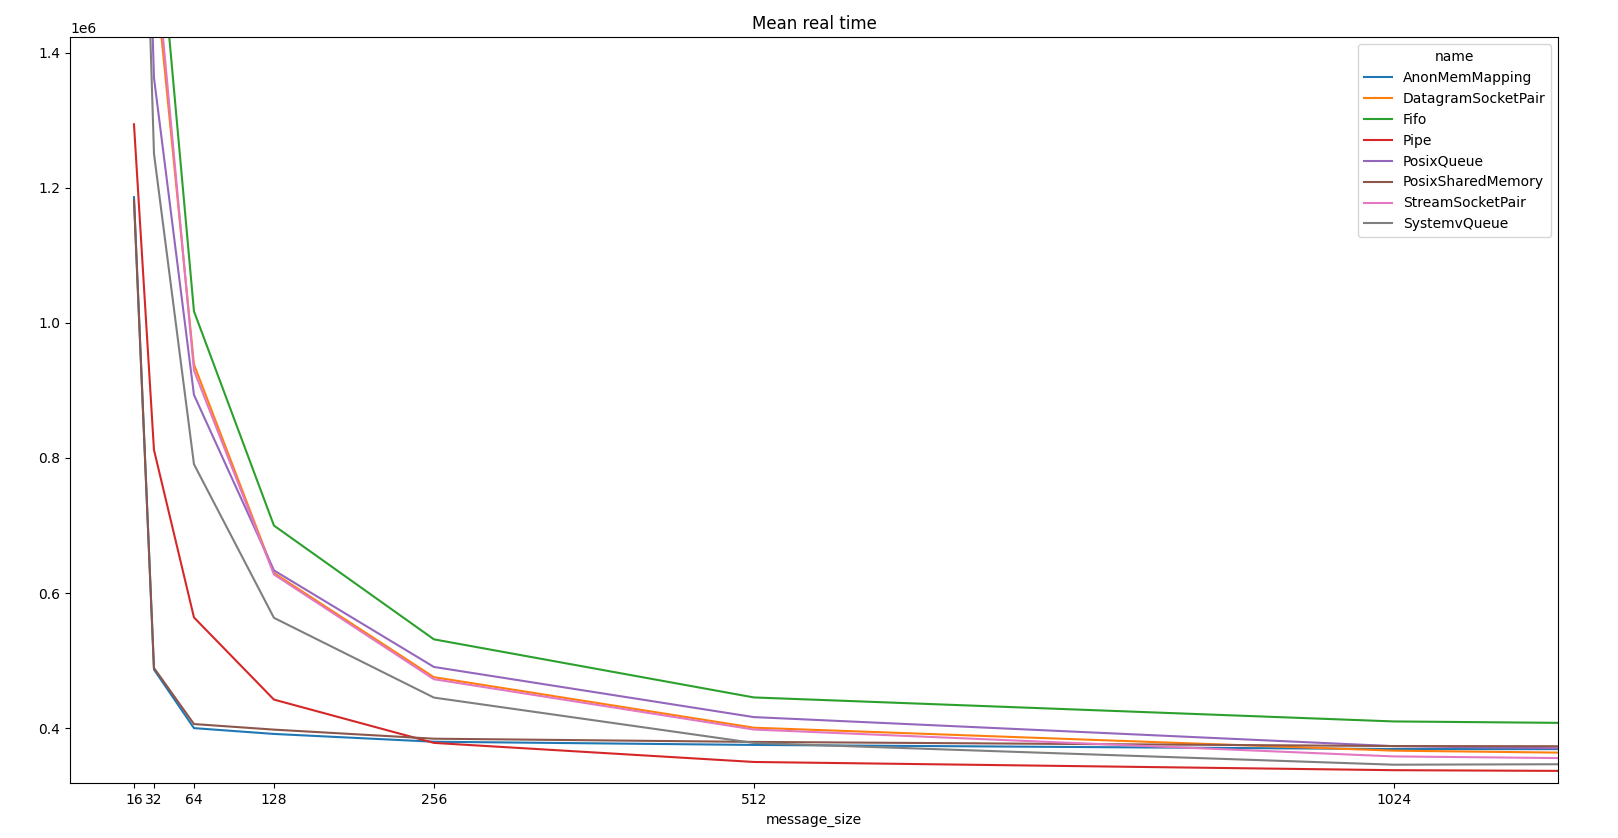
\includegraphics[width=\textwidth]{./imgs/performance.png}
  \end{minipage}
  \caption{Сравнительный график производительности средств межпроцессной
    коммуникации.}
  \label{fig:performance}
\end{figure}

Как и ожидалось, самую высокую производительность для передачи сообщений
небольшого размера показала разделяемая память и анонимная отображаемая память.
Этот отрыв обуславливается экономией на системных вызовах и лишних операциях
копирования в буфер ядра, которые присущи остальным методам межпроцессной
коммуникации.

На больших размерах буферов разницы практически не оказалось, т.к. количество
системных вызовов было сведено к минимуму.

Файловые отображения показали плохие результаты на любом размере буфера, т.к.
зависят от быстродействия персистентной файловой системы. Поэтому они были
намеренно исключены из графика сравнения на этапе подготовки данных.

Стоит упомянуть, что производительность средств межпроцессной коммуникации может
меняться от конкретной конфигурации системы и режима нагрузки, и, например,
зависеть от версии ядра Linux. Измерения приведенные в данной работе выполнены
на версии ядра \verb|6.6.52|, но могут быть легко воспроизведены на любой
целевой системе и гибко сконфигурированны под целевой режим нагрузки путем
изменения размеров и/или количества передаваемых пакетов.

\newpage
\anonsection{ЗАКЛЮЧЕНИЕ}  %Заключение

В ходе выполнения курсовой работы была разработана библиотека для реализации
межпроцессного взаимодействия на базе операционной системы Linux, проведены
тесты производительности интерфейсов данной библиотеки и на их основе оценена
производительность различных механизмов передачи данных между процессами.

Основной целью данной курсовой работы было проведение сравнительного анлиза
средств межпроцессной коммуникации в операцинной системе Linux. Результаты
выполнения задачи демонстрируют корректность реализации библиотеки, на основе
которой реализованы бенчмарки, что подтверждается автоматизированными
юнит-тестами. Разработанные тесты производительности предоставляют гибкий
инструмент для сравнения производительности методов межпроцессной коммуникации в
различных условяих и режимах нагрузки. Были получены и оценены данные о
производительности наиболее релевантных в контексте обмена информацией между
процессами интерфейсов.

В заключение, несмотря на достигнутые положительные результаты, существует
потенциал для дальнейшего улучшения библиотеки. Это включает в себя тестирование
и измерение производительности на основе различных реализаций UNIX систем, а
также расширение интерфейса для двунаправленной коммуникации.

\newpage
\renewcommand\refname{СПИСОК ИСПОЛЬЗОВАННЫХ ИСТОЧНИКОВ}
% Список литературы
\clearpage
\phantomsection
\addcontentsline{toc}{section}{\protect\numberline{}\refname}
%\bibliographystyle{ugost2008s}  %utf8gost71u.bst} %utf8gost705u} %gost2008s}
{\catcode`"\active\def"{\relax}
% \bibliography{biblio2}
\printbibliography
}
\newpage
\settocdepth{section}
\anonsection{ПРИЛОЖЕНИЕ А}
\vspace{-30pt}

\begin{listing}[H]
  \caption{Определение класса Subprocess}
  \label{lst:subprocess_declaration}
  \inputminted[style=bw, breaklines, frame=single, fontsize = \footnotesize, linenos=false, xleftmargin = 1.5em]{cpp}{./listings/subprocess_declaration.hpp}
\end{listing}

\begin{listing}[H]
  \caption{Определение методов класса FdBufIn}
  \label{lst:fdbufin_definition}
  \inputminted[style=bw, breaklines, frame=single, fontsize = \footnotesize, linenos=false, xleftmargin = 1.5em]{cpp}{./listings/fdbufin_definition.cpp}
\end{listing}

\begin{listing}[H]
  \caption{Определение методов класса FdBufOut}
  \label{lst:fdbufout_definition}
  \inputminted[style=bw, breaklines, frame=single, fontsize = \footnotesize, linenos=false, xleftmargin = 1.5em]{cpp}{./listings/fdbufout_definition.cpp}
\end{listing}

\begin{listing}[H]
  \caption{Реализация GetSyscallError()}
  \label{lst:errors_definition}
  \begin{minted}[style=bw, breaklines, frame=single, fontsize = \footnotesize, linenos=false, xleftmargin = 1.5em]{cpp}
#include <cerrno>
#include <cstring>
#include <format>

namespace stewkk::ipc {

SyscallError GetSyscallError() {
  auto err = errno;
  return SyscallError(err, std::system_category(), std::format("{}", strerrorname_np(err)));
}

}  // namespace stewkk::ipc
  \end{minted}
\end{listing}

\begin{listing}[H]
  \caption{Объявление класса Pipe}
  \label{lst:pipe_definition}
  \inputminted[style=bw, breaklines, frame=single, fontsize = \footnotesize, linenos=false, xleftmargin = 1.5em]{cpp}{./listings/pipe.hpp}
\end{listing}

\begin{listing}[H]
  \caption{Определение методов класса Pipe}
  \label{lst:pipe_declaration}
  \inputminted[style=bw, breaklines, frame=single, fontsize = \footnotesize, linenos=false, xleftmargin = 1.5em]{cpp}{./listings/pipe.cpp}
\end{listing}

\begin{listing}[H]
  \caption{Скрипт для построения графика результатов бенчмарков}
  \label{lst:plot}
  \inputminted[style=bw, breaklines, frame=single, fontsize = \footnotesize, linenos=false, xleftmargin = 1.5em]{py}{./listings/plot.py}
\end{listing}

\end{document}
